\documentclass[tikz,border=1cm]{standalone}
\begin{document}
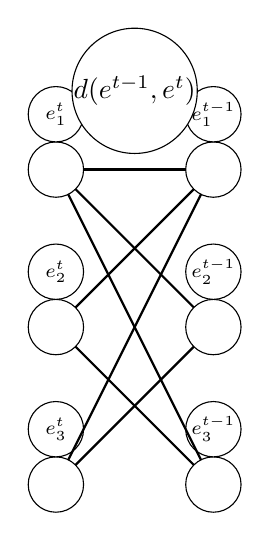
\begin{tikzpicture}[auto]
\tikzset{
    every node/.style={
        circle,
        draw=black,
        minimum size=2em,
        inner sep=0pt,
        outer sep=0pt,
        fill=white
    },
    every label/.style={
        align=center,
        font=\scriptsize
    }
}
\node (n1) at (-1,1) [label=$e_{1}^{t}$] {};
\node (n2) at (-1,-1) [label=$e_{2}^{t}$] {};
\node (n3) at (-1,-3) [label=$e_{3}^{t}$] {};

\node (n1p) at (1,1) [label=$e_{1}^{t-1}$] {};
\node (n2p) at (1,-1) [label=$e_{2}^{t-1}$] {};
\node (n3p) at (1,-3) [label=$e_{3}^{t-1}$] {};

\draw[thick] (n1) -- (n1p);
\draw[thick] (n1) -- (n2p);
\draw[thick] (n1) -- (n3p);
\draw[thick] (n2) -- (n1p);
\draw[thick] (n2) -- (n3p);
\draw[thick] (n3) -- (n1p);
\draw[thick] (n3) -- (n2p);

\node at (0,2) {$d(e^{t-1},e^{t})$};
\end{tikzpicture}
\end{document}